\section{The \emph{Hash Join} Operator}
\label{hj}
Hash join is perhaps the most commonly used join algorithm in database
systems. Here, a hash table is built on the smaller relation, and tuples
from the larger relation are used to probe for matching values in the join
column. Since we assume that all tables are completely PCM-resident, the
join here \emph{does not} require any initial partitioning stage. Instead,
we directly proceed to the join phase. Thus, during the progress of hash join, writes will be incurred during the building of the hash table,
and also during the writing of the join results.

Each entry in the hash table consists of a pointer to the corresponding
build tuple, and the hash value for the join column. Due to the
absence of prior knowledge about the distribution of join column values
for the build relation, the hash table is expanded dynamically according
to the input. Typically, for each insertion in a bucket, a new space is
allocated, and connected to existing entries using a pointer. Thus,
such an approach incurs an additional pointer write each time a new
entry is inserted.

Our first modification is to use a well-known technique of allocating
space to hash buckets in units of \textit{pages} \cite{paging}. A
page is of fixed size and contains a sequence of contiguous fixed-size
hash-entries.  When a page overflows, a new page is allocated and linked to
the overflowing page via a pointer.  Thus, unlike the conventional hash
table wherein each \emph{pair} of entries is connected using pointers,
the interconnecting pointer here is only at page granularity. Note that
although open-addressing is another alternative for avoiding pointers,
probing for a join attribute value would have to search through the
\emph{entire table} each time, since the inner table may contain
\emph{multiple} tuples with the same join attribute value.

A control bitmap is used to indicate whether each entry in a page is vacant
or occupied, information that is required during both insertion and search in the
hash table. Each time a bucket runs out of space, a new page is allocated
to the bucket. Though such an approach may lead to space wastage when
some of the pages are not fully occupied, we save on the numerous pointer
writes that are otherwise incurred when space is allocated on a per-entry basis.

Secondly, we can reduce the writes incurred due to storing of the hash values in
the hash table by restricting the length of each hash value to just a single byte. In this
manner, we trade-off precision for fewer writes. If the hash function
distributes the values in each bucket in a perfectly uniform manner, it
would be able to distinguish between $2^8 = 256$ join column values in a
bucket. This would be sufficient if the number of distinct values mapping
to each bucket turn out to be less than this value. Otherwise, we would
have to incur the penalty (in terms of latency) of reading the actual join
column values from PCM due to the possibility of false positives.

\begin{figure}[htpb]
	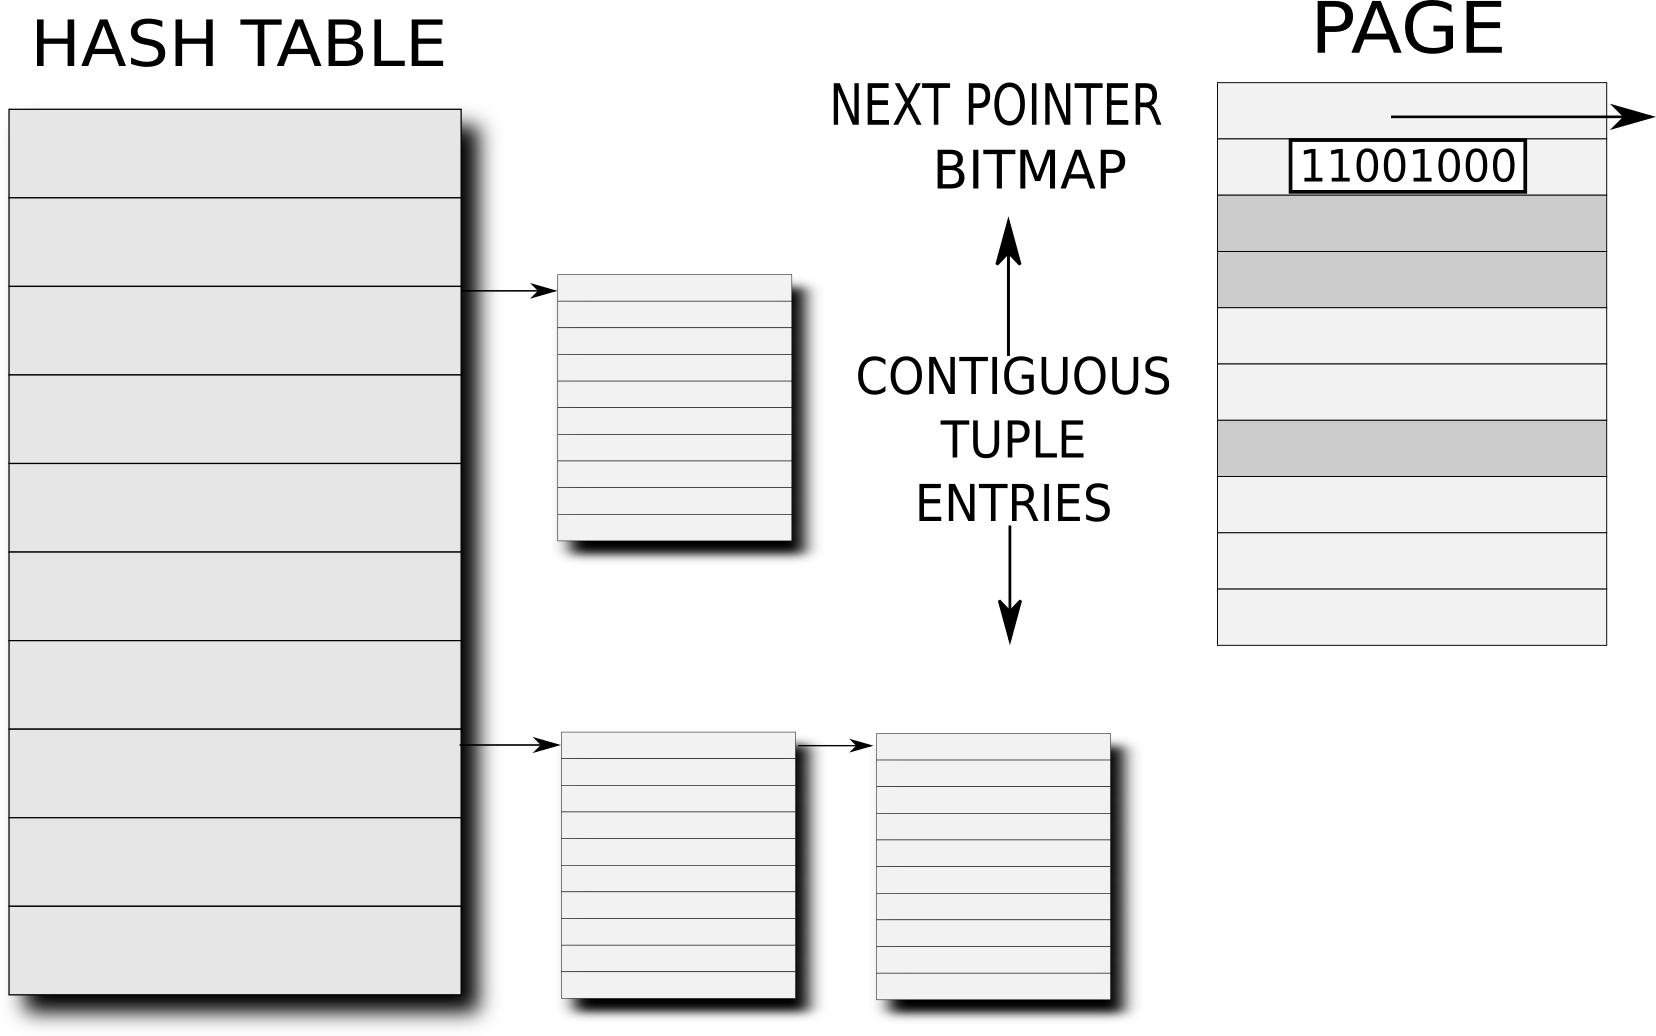
\includegraphics[height=80mm]{./fig/hash_table.png}\centering
	\caption{Paged Hash Table}
	\label{fig:hash_table}
\end{figure}

Figure~\ref{fig:hash_table} displays the hash table organization with the proposed optimizations.

\textbf{PCM write analysis}: We ignore the writes incurred while initializing each hash table bucket since they are negligible in comparison to inserting the actual entries. Assuming there are $E_{page}$ entries per page, there would now be one pointer for each $E_{page}$ set of entries. Additionally, for each insertion, a bit write would be incurred due to the bitmap update. The join tuples would also incur writes to the tune of $\hjcount \times \hjlen$. Thus, the total number of word-writes for hash join would be
$$W_{hj} = \frac{N_R \times (\hashsize +  \frac{P}{E_{page}} + \frac{1}{8} ) + \hjcount \times \hjlen }{4}$$
Since in practice both  $\frac{P}{E_{page}}$ and $\frac{1}{8}$ are small as compared to $\hashsize$, 
\vspace{-0.05in}
\begin{equation}\label{eq:hj}
 W_{hj} \approx \frac{ N_R \times \hashsize + \hjcount \times \hjlen}{4} 
\end{equation} 
